\documentclass[11pt]{article}
\date{20 de septiembre del 2019}
\usepackage{graphicx}
\usepackage[utf8]{inputenc}
\usepackage[spanish]{babel}
\usepackage{amsmath}
\usepackage{amsfonts}
\usepackage{amssymb}
\usepackage{kpfonts}
\usepackage[left=2cm,right=2cm,top=2cm,bottom=2cm]{geometry}
\usepackage{graphicx}
\graphicspath{{ENTREGABLE 1/}{Imagenes/}}
\title{\textbf{ESTACIONAMIENTOS INTELIGENTES Y PREVENTIVOS}}
\author{RUIZ TINNOCO GIOVANI DANIEL\\
		BARRERA VAZQUEZ OMAR\\
		MUÑOZ JUAREZ ALANA ANTONIO\\
		ESPARZA CABRERA JESUS DAVID\\		

\includegraphics[scale=2]{ImagenesDoc/p1.jpg} 
}

\begin{document}
\maketitle
\newpage
\section{Delitos en la sociedad}
Actualmente en la zona metropolitana de Guadalajara los diferentes tipos de delitos cometidos en sus calles, negocios y casas afectan a todos los sectores de la sociedad, la cual se ve repercutida en los ingresos que obtiene.
Los casos de inseguridad se han visto impulsados por distintos factores como los son la corrupción e impunidad al momento de impartir justicia en sus tribunales.

  Los delitos a motociclistas son unos de los repuntes que ha crecido en la actualidad, casi 8000 automotores robados al año, la mayoría retirada de sus sitios donde eran estacionadas y otros tanto a mano armada. De todos los delitos que se comenten de este tipo en especifico pocos son resueltos.
  
\subsection{Parte social del proyecto}

Año con año las ciudades inteligentes toman mas relevancia para la sociedad y según estudios del \emph{World Forum Economic} se espera cada vez mas inversión para este tipo de proyectos que resuelvan necesidades sociales desde el área tecnológica.

Nuestro proyecto se basa es los principios de la ciudades inteligentes, dar una solución a través de la tecnología disponible en las grandes urbes del siglo XXI, por lo cual se opta por proveer a centros comerciales y lugares públicos con estacionamientos inteligentes.

\subsection{Contribución social}
El asegurar un automotor es de un alto nivel de complejidad, ya que por facilidades de acceso y las pocas medidas de seguridad no garantizan evitar el robo de este tipo de transporte el cual es fácil de acceder a sus sistemas de seguridad.

\section{Proyecto para la gran urbe}
Tener en cuenta todo el contexto que genera el problema de los robos de motocicletas es propio para generar soluciones inteligentes, es ahí donde nace \emph{Estacionamientos Inteligentes y Preventivos}, de las constantes necesidades a cubrir de problemas con origen social. La idea de crear estacionamientos inteligentes se plantea como un proyecto universitario con una visión comercial, en donde se plantan las bases para hacer factible la implementación en lugares comerciales y públicos.

\subsection{Acerca del proyecto}
El proyecto consiste en la creación de plataformas inteligentes para los automotores \emph{motocicletas}, El cual emplea un anclaje inteligente por sistema de computadora que se explica a continuación las acciones correspondientes a su uso:
\begin{enumerate}
	\item El motociclista ingresa por el estacionamiento de un centro comercial o lugar publico,lo normal seria que cuando estacione el automotor sea en un lugar común para motocicletas, pero que no esta custodiado por nadie, por lo que su seguridad consistirá en utilizar un candado que se ajuste entre la llanta y las barras suspensorias del vehículo.
	\item El usuario se aleja del lugar dejando expuesta su pertenencia por un lapso que va de un corto o largo tiempo. Por lo que durante ese tiempo la motocicleta no es vigilada por nadie y tampoco esta protegida por los candados, ya que la mayoría de los robos los sujetos tienen camionetas para transportarlas sin necesidad de retirar los obstáculos en ese momento.
	\item Cuando regresa el usuario y no encuentra su automotor, inmediatamente lo reporta a los encargados de la seguridad del lugar o en algunos casos a seguridad publica. Para cuando es el momento de la reacción de los agentes de seguridad, es demasiado tarde, ya que pronto terminara siendo desmantelada en algún lugar de reventa de partes.
	\item El usuario perdió un patrimonio fundamental para el, que es muy poco probable que lo recupere o que el estacionamiento encargado le ofrezca la reparación del hecho.   
\end{enumerate}


\subsection{Proyecto en acción}
El proyecto ha trabajar contempla los aspectos mencionados en la lista anterior, cuestiones que fueron abordadas desde un contexto tecnológico y social por lo que se redacta su funcionamiento a continuación:
\begin{enumerate}
	\item El usuario al llegar al estacionamiento observa las plataformas inteligentes, las cuales tienen un espacio universal para todo tipo de motocicletas, incluso si estas han sido modificadas. El usuario estable en forma recta con la plataforma y la recarga hasta que el sensor de posición logra identificar las dos ruedas y la barra de suspensión.
	\item Una vez detectado el posicionamiento de los tres puntos de la motocicleta, el micro-controlador procederá a asegurarla con dos pernos de seguridad de alto calibre. La plataforma expedirá una tarjeta de control la cual tendrá un numero de identificación que estara cambiando constantemente y que podrá ingresar desde una aplicacion de su telefono movil o desde una pagina web.
	\item Una vez ingresando a cualquier opcion, se podra monitorear el estado del automotor, como ejemplo de opciones; rasgos de movimiento, intento de sabotaje a la maquina o incluso si se intento usar otra tarjeta que no es la correcta. Para esto es necesario la creacion de un servidor web, aplicaciones para distintos SO (sistemas operativos) y un microcontrolador sellado en el suelo.
	\item En caso de una alarma autentica, se dezplazara una pantalla con la opcion llamar a \emph{los cuerpos de seguridad}, esto con el fin de que el usuario no tenga que enfrentar a los asaltantes y de este modo exponer su integridad fisica.
	\item Esta idea parte de los beneficios planteados de manera tripartita, una recaudacion fiscal por el uso de estos aparatos, que pueden contribuir al gasto del combate a delictos del fuero comun. otra parte formaria a ser del lugar de donde pertenece el estacionamiento, en casos como plazas comerciales o edificios del gobierno asi como instituciones educativas. Y por ultimo la parte de las utilidades y de mantenimiento para la empresa encarga de la concesion.
	
\end{enumerate}
\newpage
\section{Material}
Tomar en cuenta los costos de los materiales a la hora de llevar a cabo un proyecto de innovacion en el area tecnologica, casi siempre termina en estragos por lo multiples y elevados costos que toman los fabricantes. A partir de la iniciativa de \emph{estacionamientos inteligentes y preventivos}, se considera el hacer un prototipo funcional y costos reales en el mercado, con esto sienta las bases para que se tenga un costo estimado real de lo que costaria en el mercado.

Los materiales que se consideran pueden estar o no en partes futuras del proyecto conforme a las modificaciones que este pueda sufrir. Se presenta a continuacion la tabla de estimados de precios de un prototipo funcional:

\begin{center}
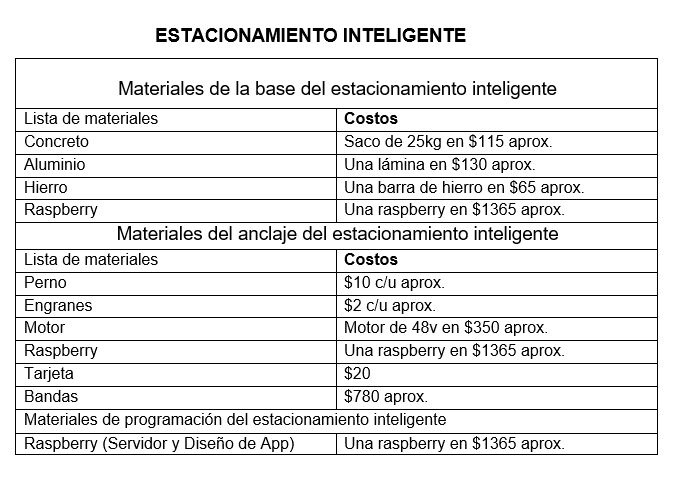
\includegraphics[scale=0.8]{ImagenesDoc/costos.JPG} 
\end{center}
\label{}
\newpage
\subsection{Relación del proyecto con las materias}
\begin{flushleft}
En este apartado hablaremos sobre como nuestro proyecto se relaciona con las diferentes materias, así mismo dar a conocer como se relacionan con el proyecto.\\
\end{flushleft}
\begin{center}
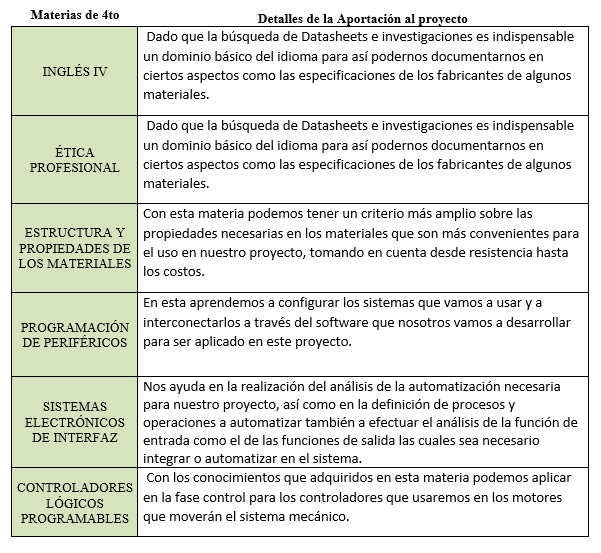
\includegraphics[scale=1]{ImagenesDoc/Aportacionesmaterias.PNG} 
\end{center}
\end{document}
